\kapitola{Metodika}
Na začátku je potřeba provést analýzu problému s ohledem na požadavky stanovené konzultacemi s vedoucím. Návrh bude také zahrnovat experimenty, které budou s neuroevolucí provedeny.

Po návrhu bude následovat implementace daného řešení. Popis řešení bude přidán do této práce. V průběhu implementace bude také kód a návrh postupně upravován na základě požadavků, které se mohou objevit až při implementaci navrženého řešení.

Po implementaci bude následovat realizace a vyhodnocení experimentů popsaných v návrhu.

Na závěr proběhne vyhodnocení řešení s návrhem možných zlepšení.
\kapitola{Analýza problému}
Tato kapitola se zabývá analýzou funkčních a nefunkčních požadavků pro softwarové řešení. Požadavky vznikaly na základě konzultace s vedoucím a vlastní invencí.

\sekce{Funkční požadavky}
Funkční požadavky jsou rozděleny do několika kategorii.

\podsekce{Simulace}
Vyhodnocování agenta bude probíhat jeho nasazením v simulovaném prostředí. Fitness bude pak vyhodnocena na základě jeho akcí v prostředí.
\begin{itemize}
	\item Testovací prostředí musí být pro všechny agenty stejné
	\item Fitness funkce musí být deterministická
	\item Fitness by měla být zjistitelná kdykoliv v průběhu simulace
	\item Simulace by měla být konfigurovatelná 
	\item Možnost změny obtížnosti simulace pro agenta
	\item Měla by existovat možnost spuštění více instancí simulace v rámci jednoho programu
\end{itemize}
\podsekce{Vizualizace}
Průběh algoritmu je třeba zobrazit.
\begin{itemize}
	\item Je třeba provést grafickou vizualizaci fyzikální simulace
	\item Při zobrazení by mělo být možné vyčíst stav agenta (fitness, senzory, ...) 
	\item Možnost vizualizace průběhu simulace v reálném čase (například pro její demonstraci v předmětu VUI2)
\end{itemize}

\podsekce{Experimenty}
Práce zahrnuje vyhodnocování agenta v různých podmínkách z tohoto vychází následující požadavky:

\begin{itemize}
\end{itemize}

\sekce{Nefunkční požadavky} 
Spolu s funkčními požadavky jsou na řešení kladeny také požadavky nefunkční.
\begin{itemize}
	% TODO: Předělat do formátu Něco - ....
	\item Škálovatelnost - Možnost spustit a vykreslit libovolné množství simulací
	\item Rychlost simulace. - Simulace by měla být schopná samostatně běžet alespoň rychlostí 30 snímků za vteřinu.
	\item Robustnost - Simulace by měla být odolná neočekávaným situacím
	\item Portabilita - bylo třeba zajistit, aby šlo kód rozběhnout v různých platformách v různých konfigurací.
	\item Robustnost - Simulace by si měla poradit s neočekávanými vstupy, jako je třeba \textbf{NaN}, který vychází z neuronové sítě.
\end{itemize}

\kapitola{Návrh řešení}


\kapitola{Implementace}
Vlastní práce se skládá ze dvou částí. Klientská část, která slouží k~vizualizaci algoritmu a zobrazení výsledků ze serverové části. Serverová část pro maximální urychlení simulace. 

\sekce{Simulace}
Simulace je realizovaná jako knihovna pro Node.js, lze jí tedy použít jak u klientské částí, tak u serverové části. Poskytuje kompletní fyzikální simulaci agenta, prostředí ve kterém se pohybuje, jeho ovládání a výpočet fitness funkce. Součástí simulačního prostředí je také kód pro její vizualizaci.

Rychlost byla zajištěna implementací profilovacího programu (\textbf{benchmark.js} ve složce simulation), který spouští simulaci na předem připravené populaci jedinců. Výstupem je pak doba, za jakou jí vyhodnotil na jednom jádře procesoru. Tento údaj byl pak používán při implementaci simulace pro orientační představu, jak moc případné změny v kódu ovlivňují rychlost samotné simulace. Dále byla simulace podrobena občasnému profilování v klientské částí pomocí vývojářských nástrojů prohlížeče chrome, na kterém simulace jede nejlépe.

Nenáročnost, která souvisí s rychlostí, pak byla zajištěna tím, že bylo v průběhu psaní kódu dbáno na to, aby v průběhu simulace nedocházelo k přebytečným alokacím, které by nejen mohly způsobit přebytečný nárůst požadované paměti, ale hrozilo by také nepředvídatelné zpomalení, které sebou přináší jazyk využívající garbage kolektor.

Robustnost je podrobněji vysvětlená v sekci \ref{sec:fitness} a popis toho, jak bylo dosaženo stejných podmínek pro všechny agenty lze nalézt v návrhu \ref{sec:ECS} především v popisu RoadManageru.

\podsekce{Fitness funkce}
\label{sec:fitness}
Fitness funkce je důležitou součástí simulace, která zásadně ovlivňuje chování výsledných agentů a je tedy nutné jí volit vhodně. Je nutné, aby funkce agenta motivovala ke správné činnosti.

Po několika pokusech a konzultaci s vedoucím práce byla jako metrika úspěchu agenta zvolena celková vzdálenost, kterou je agent schopný překonat v průběhu jedné generace. Výpočet je realizován pomocí RoadDirectoru, který si při každém přechodu zaznamená bod, ve kterém se po přesunu agent nachází. Výsledná fitness je pak součet uražených vzdáleností pro každou místnost. Road direktor si pro každou obrazovku uchovává vzdálenost, kterou agent v dané obrazovce překonal. Výsledným fitness je pak součet všech vzdáleností na všech obrazovkách.

Simulace může být také předčasně zastavena v případě, že agent koliduje s překážkou. Znemožní se mu tím získání většího skóre.

\podsekce{Simulační prostředí}
\label{sec:simulationEnvironment}
Simulační prostředí poskytuje sadu překážek, kterou agent musí překonat. Testuje se tak, co je vlastně agent schopný se naučit. V zadání práce lze nalézt podmínku pro postupné stupňování obtížnosti, tohoto je dosaženo právě změnou simulovaného prostředí. V rámci těchto požadavků byly do road direktoru na-implementovány následující dílky.

Z obrázku \ref{fig:benchmarkcluster} a tabulky \ref{tbl:benchmark} lze vyčíst, že vyhodnocení 1000 jedinců o 1000 generacích trvá něco okolo 9 h čistého výpočetního času a to do měření není započítáno to, že se agenti postupně zlepšují, což koreluje s delší dobou evaluace. 

Z tohoto důvodu bylo ověřování rozděleno do 3 částí různých obtížností. Volba obtížnosti pak probíhá volbou vhodného dílků (prostředí), který má nastavené patřičné návaznosti. Protože se dílek I objevuje v simulačním prostředí dvakrát je pro jednoduchost duplikován a jsou mu změněny patřičné navazující dílky dle obtížnosti.

První konfigurace probíhá tak, že je agent postaven doprostřed silnice ve tvaru I (obrázek \ref{fig:i}). Cílem je zjistit, zda agent je schopný naučit se jezdit (nebo alespoň couvat) rovně. V této konfiguraci je jedinou návazností (z obou možných směrů) samotný dílek I. Vzniká tak nekonečný tunel, kterým může agent cestovat.

\begin{figure}[H]
	\centering
	
\includegraphics[scale=0.5]{pieces/I}
	\caption{Silnice ve tvaru písmene I}
	\label{fig:i}
\end{figure}
  
Další stupeň testuje schopnosti agenta vyhýbat se překážkám. Agent je opět postaven do silnice ve tvaru I, ale tentokrát jsou v ní zdi, kterým se musí vyhnout (obrázek \ref{fig:iwithobstructions}). Návaznost z obou stran je opět samotný dílek (je to obdobně jako je tomu v první konfiguraci).

\begin{figure}[H]
	\centering
	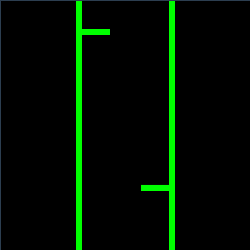
\includegraphics[scale=0.6]{pieces/I_with_obstructions}
	\caption{Silnice ve tvaru I s překážkami}
	\label{fig:iwithobstructions}
\end{figure}

Poslední Konfigurace se skládá z více dílků a testuje, zda a jak moc je schopný se agent naučit otáčet. K tomuto mu slouží malá dráha ve tvaru O skládající se z níže zobrazených dílků. Agent stejně jako v prvním případě začíná v silnici ve tvaru I s tím, že zde probíhá výše zmíněná změna návazností a to při průjezdu horní částí obrazovky je zaměněn na obrázek \ref{fig:upsidel}. V případě, že se agent vydá dolu je přesměrován na silnici ve tvaru L je tak nucen po zvládnutí jízdy dopředu naučit se zatáčet.

\begin{figure}[H]
	\centering
	
\includegraphics[scale=0.6]{pieces/upside_L}
	\caption{Silnice ve tvaru horizontálně obráceného L}
	\label{fig:upsidel}
\end{figure}

\begin{figure}[H]
	\centering
	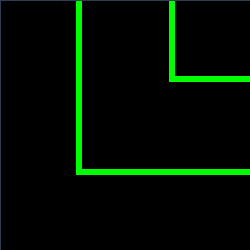
\includegraphics[scale=0.6]{pieces/L}
	\caption{Silnice ve tvaru L}
	\label{fig:l}
\end{figure}
V případě, že agent odbočí doprava je přesměrován na níže uvedený dílek ve tvaru -. Toto ověří, zda se agent dokáže přeorientovat na horizontální pohyb.
\begin{figure}[H]
	\centering
	
\includegraphics[scale=0.6]{pieces/-}
	\caption{Silnice ve tvaru -}
	\label{fig:-}
\end{figure}
Po projetí dílku ve tvaru I je přesměrován na jeden z následujících dílků.
\begin{figure}[H]
	\centering
	
\includegraphics[scale=0.6]{pieces/inverted_L}
	\caption{Silnice ve tvaru zrcadlově obráceného L}
	\label{fig:invertedl}
\end{figure}
\begin{figure}[H]
	\centering
	
\includegraphics[scale=0.6]{pieces/inverted_upside_L}
	\caption{Horizontálně a vertikálně obrácené L}
	\label{fig:invertedupsidel}
\end{figure}

\sekce{Serverová část}
Jak je jíž zmíněno v návrhu serverová část vyhodnocuje jednotlivé jedince distribuovaně s~pomocí fronty úkolů. Frontu poskytuje knihovna \textbf{Bull}, která používá \textbf{Redis} pro správu údajů o~jednotlivých úkolech. 

Cílem byla implementace robustního systému, který v~ideálním případě rozloží výpočetní zátěž mezi jednotlivé uzly rovnoměrně. Dalším požadavkem byla možnost odpojení kdykoliv kteréhokoliv z počítačů, jelikož ne všechny počítače je možné mít puštěné po celou dobu vyhodnocování.
Samotná implementace je dle návrhu rozdělena do dvou částí a to klientské části (implementace ve složce client), která obaluje algoritmus NEAT a posílá genomy na serverovou část. Serverová část obaluje simulaci a vyhodnocuje genomy na základě jejích konfigurace.

\podsekce{Konfigurovatelnost}
Experimenty, které bude klientská část provádět jsou nastavitelné s pomocí dvou konfiguračních souborů.
Globální konfigurační soubor \emph{config.env}, který nastavuje proměnné prostředí umožňuje nastavit jedinou proměnnou a to FPS, která řídí jednotný krok simulačního enginu. Fixní krok je tu proto, aby se zajistilo, že všechny simulace běžely ve stejných podmínkách.

Druhým jíž zajímavějším konfiguračním souborem je \emph{batch.json}. Tento soubor obsahuje informace o všech experimentech, které se mají spustit. Data o každém experimentu jsou uchována v jednoduchém JSON objektu, který obsahuje následující informace:

\begin{itemize}
	\item Nastavení knihovny Neataptic:
	\begin{itemize}
		\item INPUTS - Počet neuronů ve vstupní vrstvě ,
		\item OUTPUTS - Počet neuronů ve výstupní vrstvě
		\item POPSIZE - Velikost populace
		\item MUTATION\_RATE - Pravděpodobnost mutace
		\item ELITISM - Zkopíruje beze změny N nejlepších jedinců
		\item EQUAL - Při zapnutí vede k větší diverzitě s ohledem na architekturu výsledných neuronových sítí
	\end{itemize}
	\item Nastavení simulace
	\begin{itemize}
		\item STARTING\_PIECE - Dílek na kterém agent začíná. Jejích popis lze nalézt v RoadManageru
		\item OPTIONS - Umožňuje zapnout některé z rozšíření (popsaných v kapitole \ref{sec:extensions}). Následující možnosti
		\begin{itemize}
			\item holdWheel - Možnost držení volantu ve fixní pozici
			\item inputVelocity - Přidává na vstup neuronové sítě aktuální rychlost
			\item inputWheel - Přidává na vstup neuronové sítě aktuální náklon volantu
		\end{itemize}
		\item TIME - Počet vteřin, který určuje maximální dobu simulace
	\end{itemize}
\end{itemize}

\podsekce{Výpočetní cluster}
\label{sec:cluster}
Ukázalo se, že vyhodnocování simulace zabírá neúměrné množství času a to i na nejvýkonnějším dostupném počítači.

Například vyhodnocení jedné generace populace o~1024 jedincích zabralo ~60 s~na nejsilnějším dostupném pc. Z~tohoto důvodu bylo rozhodnuto o~distribuci výpočetní zátěže mezi více počítačů. Byl vytvořen výpočetní cluster se specifikací popsanou v~tabulce \ref{table:hw_table}.
\begin{table}[h!]
	\centering
	\begin{tabular}{|l|c|c|c|}
		\hline 
		Procesor & RAM & Počet & Architektura\\ 
		\hline 
		S5P6818 Octa core & 1 GB & 2 & arm64 \\ 
		\hline 
		Broadcom BCM2837B0 quad-core & 1 GB & 1 & arm32 \\ 
		\hline 
		Phenom X4 965 & 8 GB & 1 & x64 \\ 
		\hline
		Intel Core i5-2300 & 4 GB & 1 & x64 \\ 
		\hline 
		Intel atom x5-Z8350 & 2 GB & 1 & x64 \\ 
		\hline
		Cortex-A5 & 1 GB & 1 & armv7l \\
		\hline
	\end{tabular} 
	\caption{Použitý hardware}
	\label{table:hw_table}
	
\end{table}

Lze i namítnout, že se zde projevuje určitá režie při síťové komunikaci se serverem, což může být zdrojem určitého zpomalení.

Pro ověření rychlosti bylo provedeno měření výkonu clusteru a jeho porovnání s nejvýkonnější dostupnou sestavou. Měření bylo provedeno nad náhodně vygenerovanými populacemi. Jelikož se simulace může ukončit předčasně (například při kolizi s překážkou), byla simulace provedena pro každou velikost $10\times$ a výsledek byl zprůměrován. Naměřená data lze nalézt v tabulce \ref{tbl:benchmark} ze které vychází obrázek \ref{fig:benchmarkcluster} na kterém lze vidět výsledky tohoto srovnání. 

Porovnání rychlosti clusteru s nejvýkonnějším dostupným počítačem ukazuje, že cluster je ve většině případů skoro stejně nebo  výrazně rychlejší než samostatný výpočet. Jediné dvě naměřené instance, kde toto neplatí, je u populací o velikosti 100 a 200, kde si cluster vede mírně hůře, než nejvýkonnější dostupná sestava.

Toto lze vysvětlit jak přítomností méně výkonného hardwaru v clusteru (především se jedná o S5P6818) na které se musí u menších populací čekat. Pro ověření této teorie byl cluster spuštěn v dalších konfiguracích, kde byly postupně odebírány jednotlivé počítače a měření bylo opakováno. 

\begin{itemize}
	\item Cluster - Celý cluster
	\item Cluster-2 - Odebrán S5P6818 (obě jednotky)
	\item Cluster-3 - Odebrán Intel atom x5-Z8350
	\item Cluster-4 - Odebrán AMD A4-4300M
\end{itemize}
\begin{table}[H]
	\begin{tabular}{|l|c|c|c|c|c|}
		\hline
		Jedinců & Cluster & Cluster-2 & Cluster-3 & Cluster-4 & Phenom II X4 965 \\
		\hline
		100     & 9.853   & 6.1684    & 3.6887    & 3.7583    & 6.5186           \\
		\hline
		200     & 13.3993 & 9.126     & 6.451     & 7.1599    & 10.9839          \\
		\hline
		300     & 15.5628 & 10.5351   & 9.08      & 10.8206   & 16.8723          \\
		\hline
		400     & 17.7699 & 13.6263   & 11.9285   & 13.0231   & 23.5019          \\
		\hline
		500     & 19.1542 & 14.303    & 15.349    & 16.3707   & 31.7831          \\
		\hline
		600     & 20.4675 & 18.8677   & 18.571    & 20.0113   & 37.3242          \\
		\hline
		700     & 23.4671 & 20.1617   & 20.9039   & 23.7305   & 40.66            \\
		\hline
		800     & 25.07   & 23.3143   & 24.9978   & 26.3178   & 44.8019          \\
		\hline
		900     & 29.3611 & 28.1234   & 26.6288   & 29.6816   & 52.8829          \\
		\hline
		1000    & 30.5498 & 28.7635   & 29.5586   & 33.5195   & 62.8967          \\
		\hline
		1100    & 32.2825 & 32.0137   & 30.7372   & 37.2753   & 65.2363          \\
		\hline
		1200    & 34.3818 & 31.8152   & 34.0371   & 42.1325   & 72.2926          \\
		\hline
		1300    & 37.3422 & 35.8219   & 37.4416   & 40.3347   & 75.2937          \\
		\hline
		1400    & 38.4452 & 41.3896   & 38.6274   & 41.3493   & 81.1193          \\
		\hline
		1500    & 40.0487 & 43.225    & 43.4606   & 43.9233   & 81.3101 \\    
		\hline     
	\end{tabular}
	\caption{Naměřená data}
	\label{tbl:benchmark}
\end{table}
Je nutné však podotknout, že proměnlivá doba u vyhodnocování jedince znamená, že měření není zcela přesné. Nicméně lze na základě dat usoudit, že u větších populací dochází k přibližně $2\times$ zrychlení.

\begin{figure}[H]
	\centering
	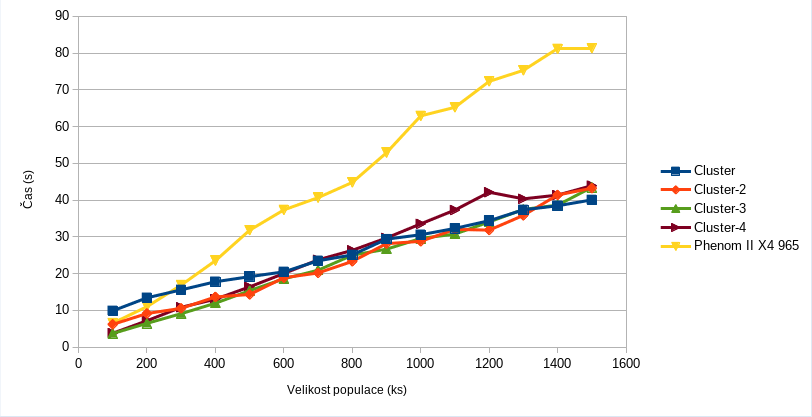
\includegraphics[scale=0.7]{benchmarkCluster}
	\caption{Porovnání rychlosti clusteru s jedním PC}
	\label{fig:benchmarkcluster}
\end{figure}

\podsekce{Docker swarm}
Pro snadnou distribuci a správu byly všechny počítače zorganizovány do docker swarmu. Docker swarm obsahoval jednoho manažera (Broadcom BCM2837B0 quad-core), který zároveň spouštěl klientskou aplikaci a další služby:

Na manažeru nebyl spuštěn zpracovatel, aby se zabránilo jeho přetížení (manažer swarmu by měl být vždy dostupný).

Použití docker swarmu umožňuje především snadné nasazení a správu zpracovávajících procesů. Zároveň zajišťuje, že všechny instance zpracovatelů mají unifikovanou konfiguraci, což je zvláště důležité pro dosažení konzistentních výsledků.

\begin{figure}[H]
	\centering
	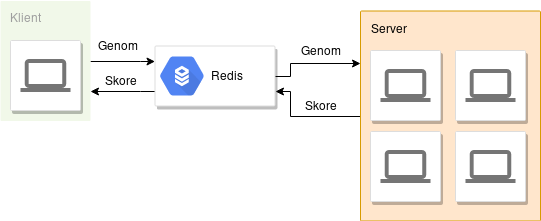
\includegraphics[scale=0.5]{distributed}
	\caption[Schéma distribuovaných výpočtů]{Schéma distribuovaných výpočtů}
	\label{fig:distributed}
\end{figure}

Tento přístup má několik výhod a to:

\begin{enumerate}
	\item Robustnost - Pokud jeden nebo více zpracovatelů selže (je například odpojen ze sítě) je možné pokračovat ve vyhodnocování (neúspěšný úkol lze vrátit zpátky do fronty). Toto v kombinaci s výše zmíněným docker swarmem znamená, že jakýkoliv výpočetní uzel lze kdykoliv vypnout a po znovu zapojení do sítě si načte nejnovější konfiguraci a začne znovu vyhodnocovat bez potřeby jakékoliv manipulace s jakoukoliv částí swarmu.
	\item Dobré rozložení zátěže - Jelikož si zpracovatel vytahuje úkoly z~fronty, je vždy optimálně zatížen, a není třeba řešit rozložení mezi různě výkonnými a zatíženými počítači.
	\item Škálovatelnost - problém lze škálovat až do doby, kdy počet procesorů nepřesáhne počet potřebných simulací. Chceme-li tedy vypočítat generaci o tisíci jedincích můžeme na ně nasadit až tisíc procesorů.
\end{enumerate}

\podsekce{Problémy implementace}
\label{sec:ImplementationTroubles}
Při implementaci serverové části a přehrávače byl objeven zásadní problém. Při vložení výsledného genomu do přehrávače se v některých případech rozcházela výsledná fitness agenta s fitness, která byla naměřena v přehrávači. 

Tuto odchylku lze vysvětlit nevyhnutelnou přítomností výpočtů, které potřebují čísla s plovoucí desetinnou čárkou, kterou vyžaduje hlavně použitý fyzikální engine a výpočty, které probíhají při vyhodnocování výstupů z neuronové sítě a to z několika důvodů:

Ačkoliv je standard IEEE-754 deterministický nezaručuje stejný výsledek na rozdílném HW a už vůbec ne na HW v rozdílných architekturách. Problém může například nastat u volby zaokrouhlovacího módu, kterých standard IEEE-754 definuje několik a které mírně ovlivňují výslednou hodnotu.

Standard JavaScriptu nespecifikuje přesnou implementaci trigonometrických funkcí, které se hojně používají u vektorové algebry, která se opět využívá hlavně u výpočtů fyzikálního enginu.

I přes to, že odchylky způsobené výše uvedenými jevy jsou relativně malé je třeba myslet na to, že se akumulují s časem a také na to, že řídící neuronová síť se může za velmi obdobných podmínek zachovat diametrálně odlišně.

\podsekce{Monitorování stavu}
Pro monitorování stavu algoritmu byla použita webová aplikace Grafana. Jak jíž bylo řečeno v sekci \ref{sec:grafana} jedná se o nástroj pro snadnou vizualizaci dat v databázi. V případě této práce posloužila k vytvoření jednoduchého kontrolního panelu, který obsahoval následující informace:

\begin{itemize}
	\item Graf zobrazující fitness nejlepšího/nejhoršího jedince dle generací
	\item Textové pole, které obsahuje nejlepší genom
	\item Numerické pole, které obsahuje počet generací
	\item Textové pole s konfigurací v jsonu
\end{itemize}
\begin{figure}[H]
	\centering
	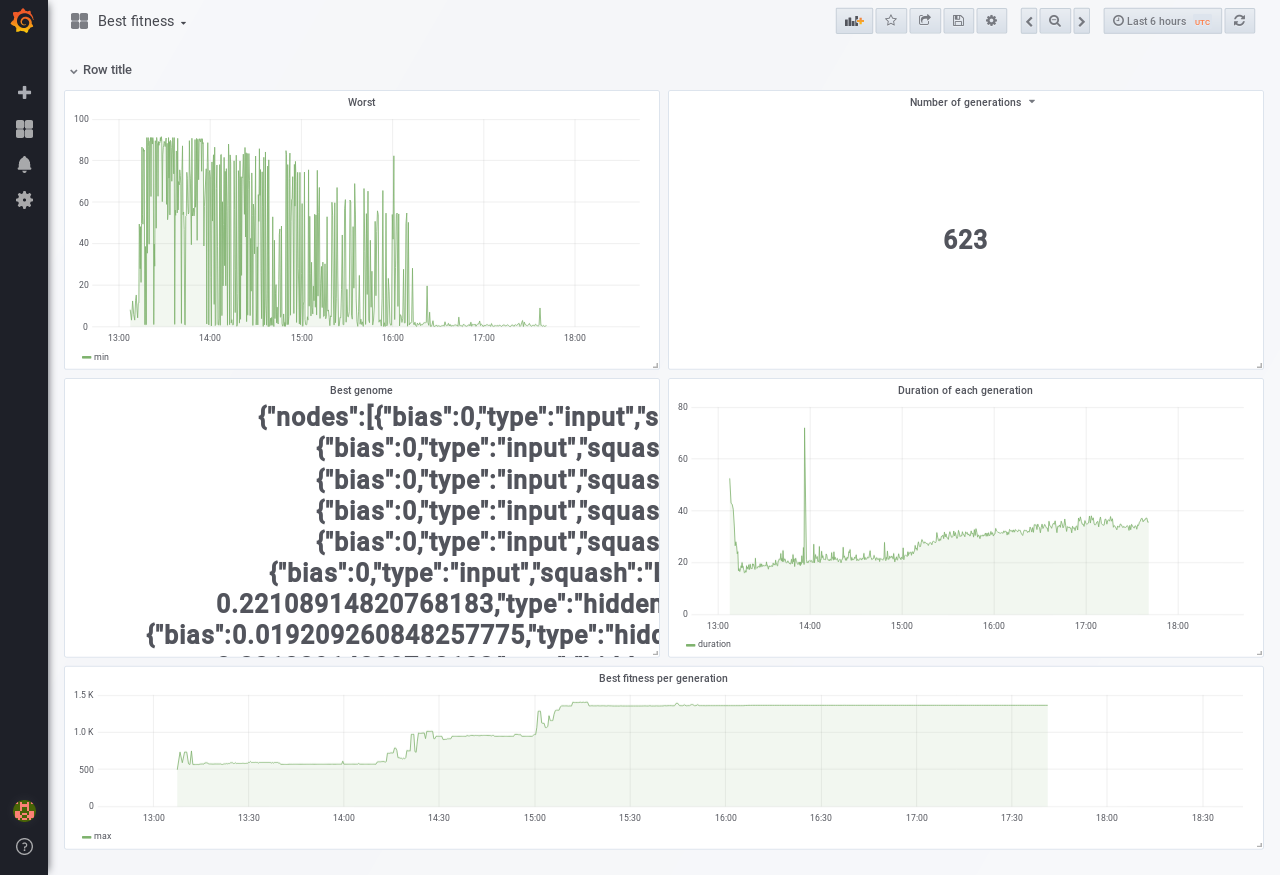
\includegraphics[width=0.6\linewidth]{grafana}
	\caption{Kontrolní panel v aplikaci grafana}
	\label{fig:grafana}
\end{figure}

Serverová část má možnost vyhodnocovat více konfigurací zároveň, toto je reflektováno v návrhu kontrolního panelu, který umožňuje nejen zobrazovat a porovnávat jednotlivé konfigurace ale také dle nich filtrovat. Toto probíhá s pomocí menu v levém horním rohu.

\sekce{Uživatelská část}
Uživatelská část byla navržena tak, aby byla schopná vizualizovat průběh algoritmu NEAT a zároveň měla možnost znovu vyhodnocení existujících genomů vygenerovaných serverovou částí. První požadavek vznikl na základě konzultace s vedoucím, který chtěl algoritmus NEAT demonstrovat v hodinách předmětu VUI2. Druhý požadavek vznikl z důvodu potřeby vizualizace řešení, které generoval sever.

Klientská část je implementovaná jako \textbf{VUE.js} aplikace realizovaná s pomocí 3 rozdílných komponent. Kromě uvedených obrazovek se jedná o komponentu \emph{Simulation}, která obaluje samotnou simulaci a vykreslování agenta. Používá jí jak přehrávač, tak vizualizace v realném čase.
\podsekce{Vizualizace}
Vizualizace se skládá z jednoduchého rozhraní, které lze vidět na obrázku \ref{fig:visualization}. V horní části je graf, zobrazující průběh genetického algoritmu. Lze v něm nalézt fitness nejlepšího, nejhoršího a průměrného jedince v populaci.

Další část se skládá z konfigurovatelného množství simulačních prostředí. Jednotliví jedinci v generaci jsou pak rovnoměrně rozloženi mezi všechna simulační prostředí a uživatel může pozorovat vývoj jedinců v reálném čase.

Poslední tlačítko slouží k urychlení simulace. Způsobí to, že se simulace začne obnovovat bez vykreslování. Toto jí značně zrychlí.

\begin{figure}[h!]
	\centering
	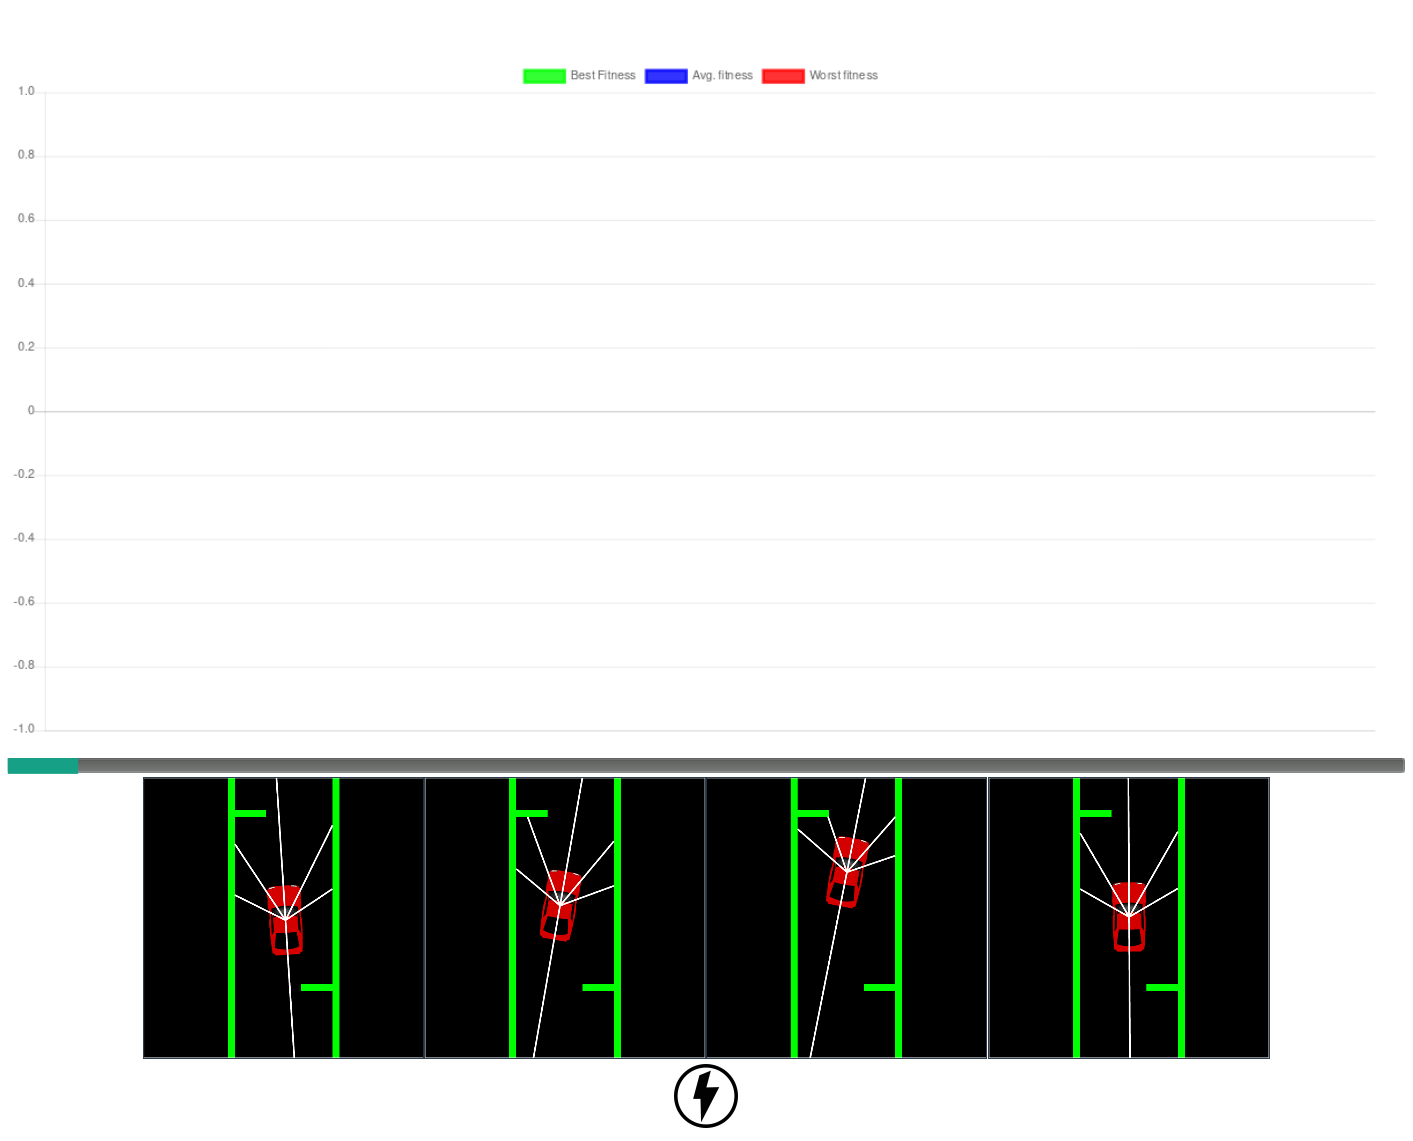
\includegraphics[width=0.6\linewidth]{visualization}
	\caption{Uživatelské rozhraní klientské části}
	\label{fig:visualization}
\end{figure}

\podsekce{Přehrávač}
Přehrávač genomů také poskytuje jednoduché rozhraní skládající se z textové částí pro vložení genomu (výstup ze serverové části lze zobrazit například v grafaně), graf pro zobrazení průběhu fitness agenta a vykreslovací část, která zobrazuje, jak si agent vedl. Pro menší výpočetní nároky je do grafu zapisována fitness každou vteřinu.  Výsledná komponenta se nachází na obrázku \ref{fig:player}.

Díky problémům s implementací naznačených v sekci \ref{sec:ImplementationTroubles} bylo třeba vymyslet alternativní způsob přehrávání. Nakonec byl návrh pozměněn tak, že si serverová část ukládá pro každý snímek pozice, úhel, aktuální fitness a dílek na kterém se agent nachází, kterou pak přehrávač interpretuje oproti klasickému přístupu, který by zahrnoval opětovnou simulaci agenta se stejným genomem. Tímto je dosaženo toho, že si lze zobrazit průběh agenta tak, jak tomu bylo při jeho vyhodnocování.

\begin{figure}[H]
	\centering
	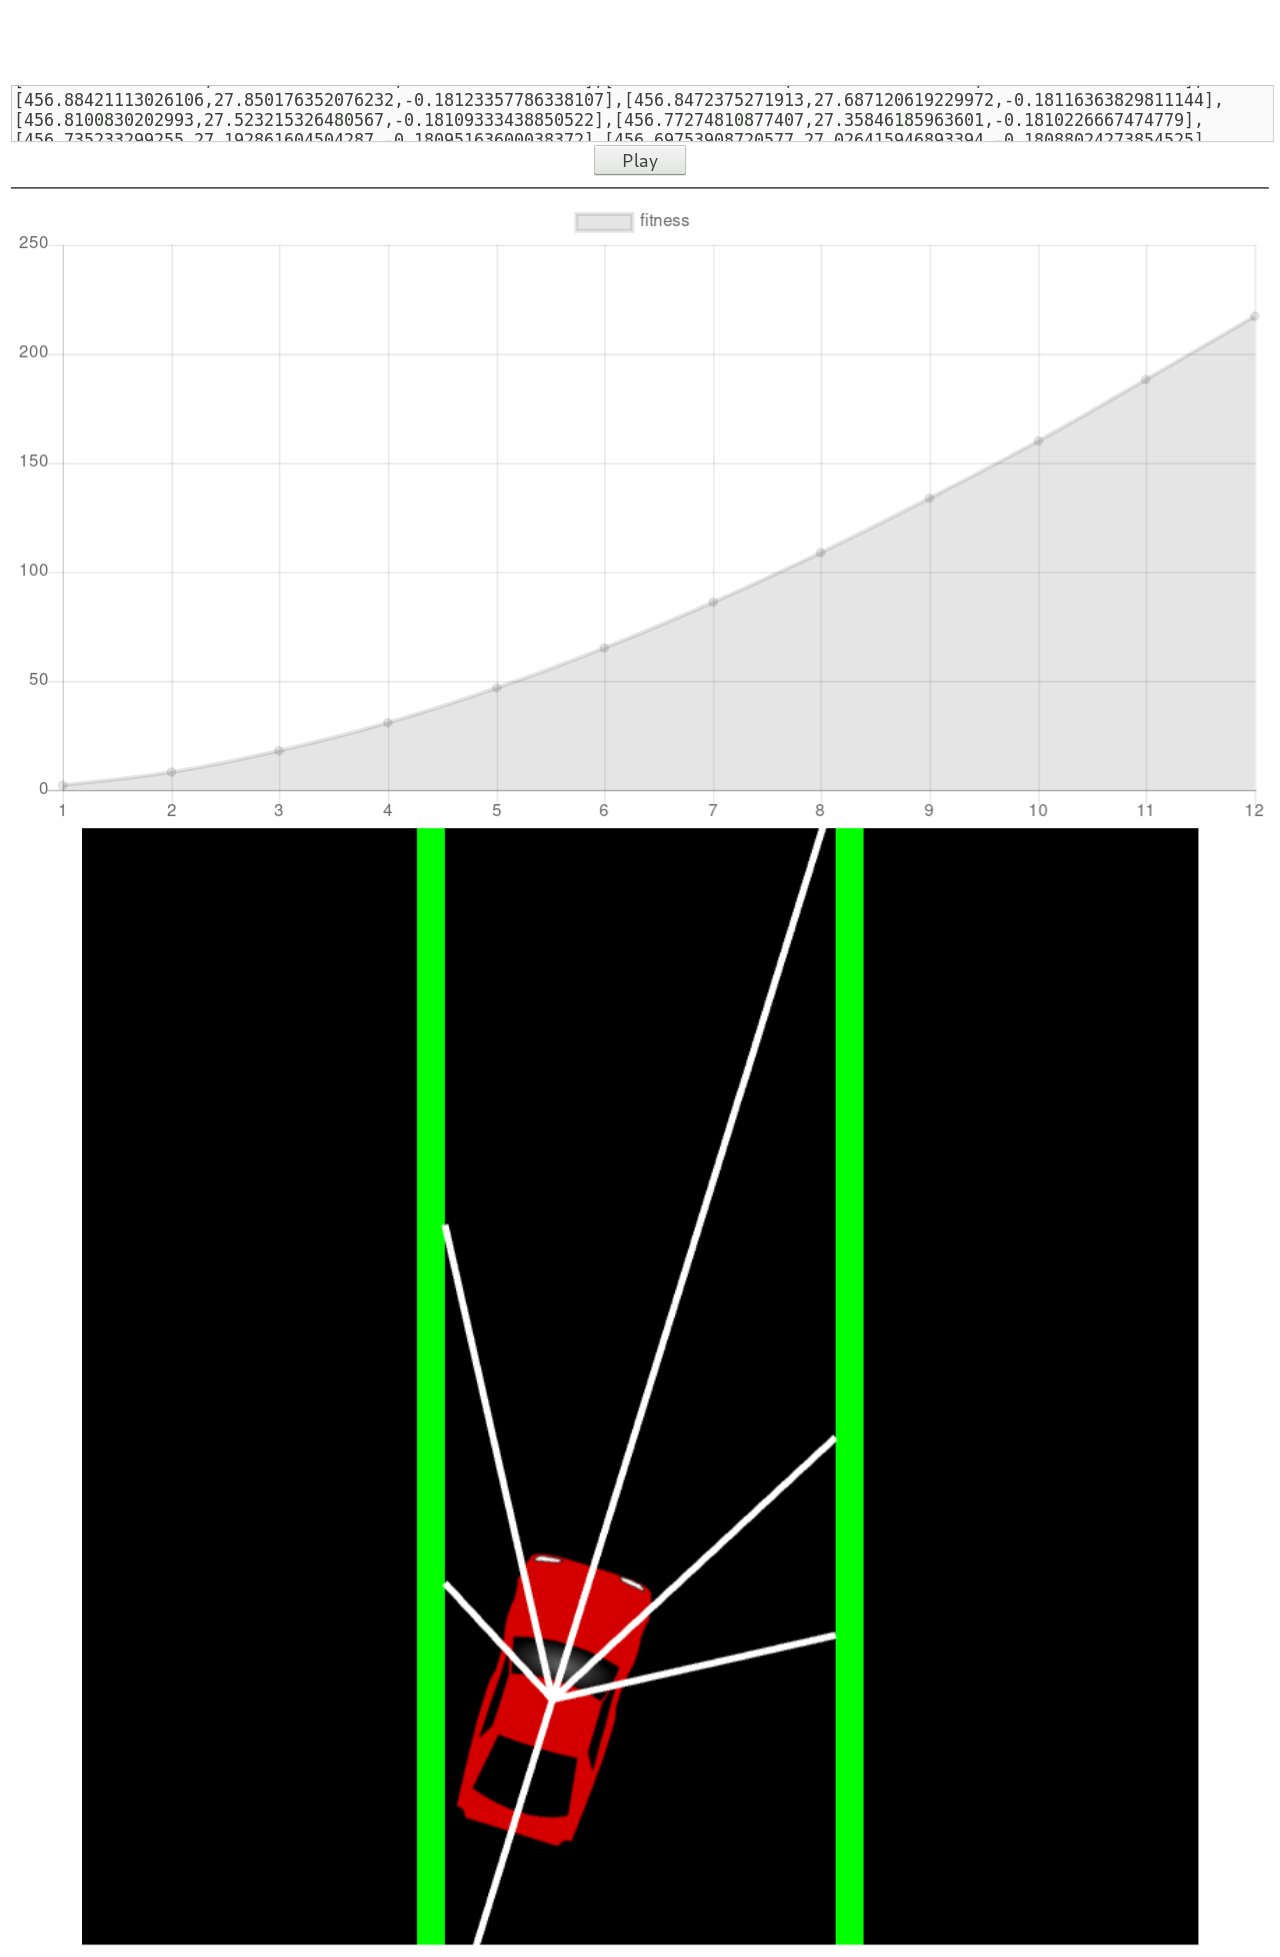
\includegraphics[width=0.5\linewidth]{player}
	\caption{Rozhraní přehrávače}
	\label{fig:player}
\end{figure}


\sekce{Nasazení serverové části}
Jak jíž bylo zmíněno serverová část je obalená do docker kontejneru jednak pro snadné nasazení a jednak z důvodu zahrnutí do swarmu.	

Nejdříve je potřeba vytvořit swarm. Tohoto lze dosáhnout zadáním příkazu \emph{docker swarm init} na počítači, který chceme používat jako swarm manager (lze také použít docker-machines a výpočty dělat na jednom počítači). Po jeho zadání se vytvoří docker swarm a zároveň je vypsán příkaz, který lze použít pro připojení dalších uzlů do swarmu (lze ho zobrazit i později s použitím příkazu \emph{docker swarm join-token worker}).

Nasazení probíhá nejdříve spuštěním příkazu \emph{docker-compose up} ve složce \textbf{client}. Toto kromě samotného klienta spustí jak následující služby:
\begin{itemize}
	\item Databáze
	\begin{itemize}
		\item Redis - pro \textbf{Bull}
		\item Postgresql - pro ukládání informací o průběhu algoritmu
	\end{itemize}
	\item Služby pro monitorování
	\begin{itemize}
		\item Grafana (port 3000) - pro monitorování stavu algoritmu NEAT
		\item Arena (port 4567) - pro monitorování stavu \textbf{Bull}
		\item Portainer (port 9000) - pro monitorování swarmu
		\item Adminer (port 8080) - pro správu databáze
	\end{itemize}
\end{itemize}
Po úspěšném provedení tohoto příkazu je třeba spustit zpracovatele na jednotlivých uzlech swarmu. Lze toho dosáhnout přechodem do složky \textbf{Server} a spuštěním příkazu \emph{docker deploy Server --compose-file docker-compose.yml}. Protože je tento příkaz v době psaní práce označen jako experimentální je třeba ho povolit. Tohoto je dosaženo modifikací souboru \textbf{daemon.json} (na linuxu je ho nutné vytvořit v \emph{/etc/docker/daemon.json}) přidáním řádku \emph{"experimental": true}.

Po tomto kroku je třeba ještě nastavit správnou ip adresu a port \textbf{Redis} serveru (ip adresa swarm mangeru) v souboru \emph{config.env}.

Po provedení těchto kroků je na každém uzlu spuštěn vyhodnocovatel, který začne automaticky stahovat a vyhodnocovat jednotlivé jedince. V případě vypnutí/pádu uzlu je úkol po čase vrácen do fronty a vyhodnocení probíhá na jiném uzlu.
\podsekce{Grafana}
Grafana vyžaduje další nastavení v podobě naimportování použitého kontrolního panelu a nastavení databázového zdroje.

Exportovaný kontrolní panel, který je k nalezení v příloze diplomové práce lze naimportovat z menu \emph{Dashboards}->\emph{manage}, které se nachází v levém kontrolním panelu. 

Přihlašovací údaje do PostgreSQL serveru jsou k nalezení také v příloze. 

\sekce{Nasazení uživatelské části}
Uživatelskou část lze jednoduše nasadit s pomocí manageru závislostí \emph{npm}. Stačí ve složce s implementací spustit příkaz (po nainstalování závislostí) \emph{npm run dev} a pak si v prohlížeči otevřít adresu \emph{localhost:8080}. V případě přehrávače je to \emph{localhost:8080/\#/player}

\kapitola{Experimenty}
Po návrhu simulačního prostředí byl agent vyzkoušen v~několika situacích se stupňující se obtížností. Každá simulace probíhala se~100 jedinci do té doby než se fitness funkce u všech stabilizovala po dostatečně dlouhou dobu. Toto trvalo 400 generací a přibližně 20 hodin čistého výpočetního času. Doba vyhodnocování byla nastavena na 120 vteřin. Volba ostatních ostatních hyper-parametru proběhla na základě empirických zkušeností získaných v průběhu implemetnace. 

Ačkoliv je pravděpodobné, že by delší doba evaluace by pravděpodobně vyústila v lepší výsledky její výpočet v různých konfiguracích se ukázal jako příliš časově náročný, navíc empirické pozorování ukázalo, že tato konfigurace poskytuje dostatečně dobré výsledky za snesitelný čas. 

S ohledem na časovou náročnost výpočtů byly zkoušeny jen konfigurace popsané v návrhu (sekce \ref{sec:extensions}) na implementovaných dílcích k náhledu v sekci \ref{sec:simulationEnvironment}.

V rámci časové úspory je každý stupeň testován jen 2x. První pokus probíhá jakýchkoliv rozšíření (vstupů/výstupů) a poté zopakován se všemi dostupnými. Cílem je zjistit, jak moc tato rozšíření ovlivňují výsledného agenta.

\sekce{První stupeň - silnice ve tvaru I}
Silnice ve tvaru I byla v obou případech agentem úspěšně překonána. Je zajímavé, že ačkoliv byl výsledný pohyb agenta stejný (relativně rovná jízda dozadu) jsou zde odlišnosti ve výsledných neuronových sítí agenta v obou konfiguracích.
\podsekce{Konfigurace bez rozšíření}
Konfigurace bez rozšíření vygenerovala agenta, který jede dozadu a reguluje směr jízdy mírným kývavým pohybem. 
Z průběhu fitness funkce je vidět, že agent dosáhl dobrých výsledků jíž v druhé generaci. Další generace přibývaly výsledné neuronové sítě na komplexnosti bez větší změny v chování agenta a fitness.
\begin{figure}[H]
	\centering
	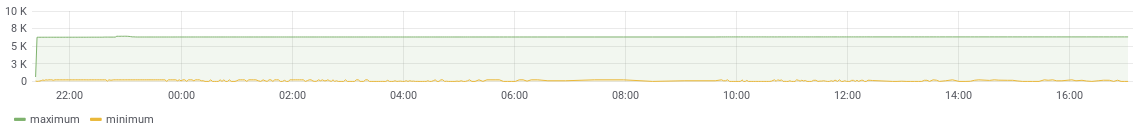
\includegraphics[width=1.0\linewidth]{solutions/Ibasic/basicGraph}
	\caption{Průběh evaluace - I bez rozšíření}
	\label{fig:basicgraph}
\end{figure}
Na výsledné neuronové síti je zajímavá zpětná vazba u prostředního oranžového neuronu s aktivační funkcí tanh, která se pravděpodobně stará o onen kývavý pohyb.
\begin{figure}[H]
	\centering
	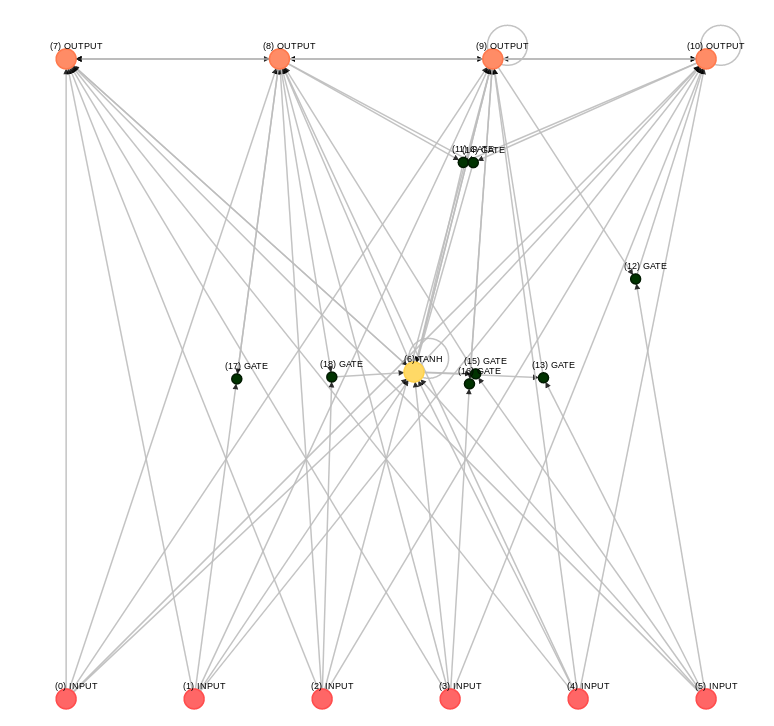
\includegraphics[width=0.6\linewidth]{solutions/Ibasic/basic}
	\caption{Neuronová síť - I bez rozšíření}
	\label{fig:basic}
\end{figure}

\podsekce{Konfigurace s rozšířeními}
Konfigurace s rozšířením byla i díky možnosti držení volantu ve fixní poloze schopná okamžitě najít možné řešení.
\begin{figure}[H]
	\centering
	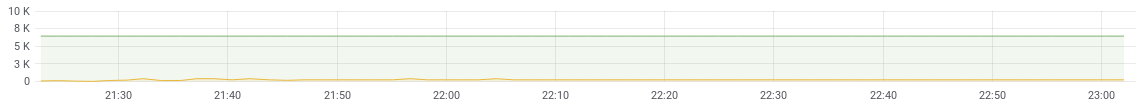
\includegraphics[width=1.0\linewidth]{solutions/Ibasic/advancedGraph}
	\caption{Průběh evaluace - I s rozšířeními}
	\label{fig:IbasicAdvancedGraph}
\end{figure}
Ve finální verzi přidala neurony do skryté vrstvy. Není jisté, zda jsou vůbec k něčemu dobré, protože pro řešení této úlohy stačí v dané konfiguraci pouze přidat plyn dozadu/dopředu a držet volant.
\begin{figure}[H]
	\centering
	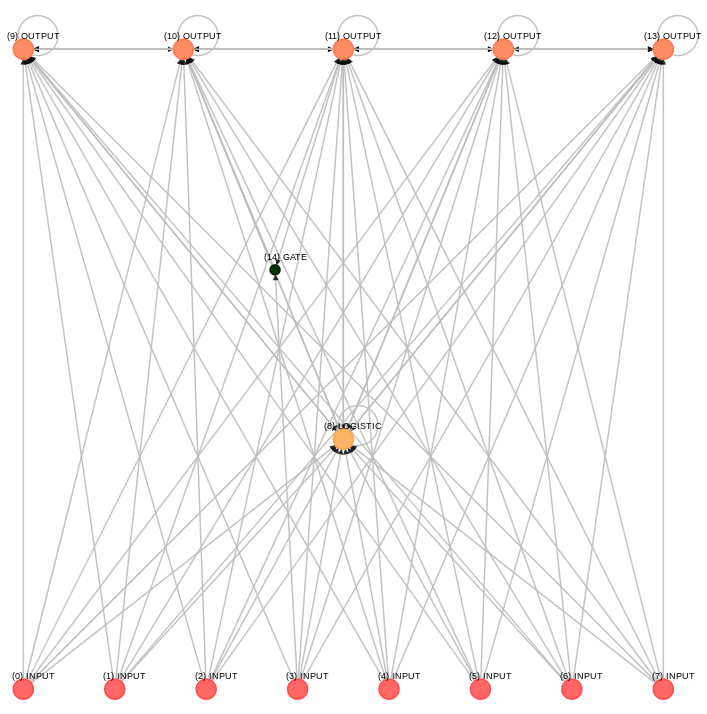
\includegraphics[width=0.6\linewidth]{solutions/Ibasic/advanced}
	\caption{Neuronová síť - I s rozšířeními}
	\label{fig:basicAdvanced}
\end{figure}

\sekce{Druhý stupeň - silnice ve tvaru I s překážkami}
Druhý stupeň obtížnosti už dělal agentovi větší problém a nepodařilo se za daný časový limit vyvinout agenta, který by ho překonal bez kolize. V tomto stupni je také vidět velký rozdíl mezi konfigurací s rozšířeními a bez rozšíření. Konfigurace s rozšířeními si totiž vedla značně lépe.
\podsekce{Konfigurace bez rozšíření}
Na první obrazovce si agent vedl docela dobře. Překážky obešel obdobným kývavým pohybem, jako je tomu u první verze, nicméně po přechodu na další obrazovku neuspěl a narazil do zdi.
\begin{figure}[H]
	\centering
	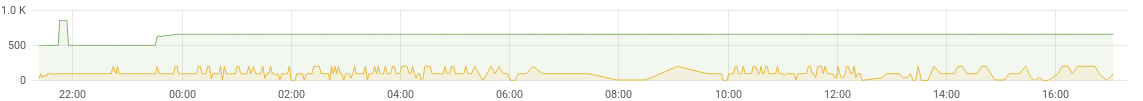
\includegraphics[width=0.7\linewidth]{solutions/IWithObstructions/basicGraph}
	\caption{Graf průběhu fitness - bez překážek}
	\label{fig:obstructionsBasicgraph}
\end{figure}
Na výsledné neuronové síti je zajímavá přítomnost neuronu s aktivační funkcí absolutní hodnota, který by mohl hrát roli právě ve vyhýbání se překážkám. Mohl by totiž sloužit jako přepínač pro zatáčení.
\begin{figure}[H]
	\centering
	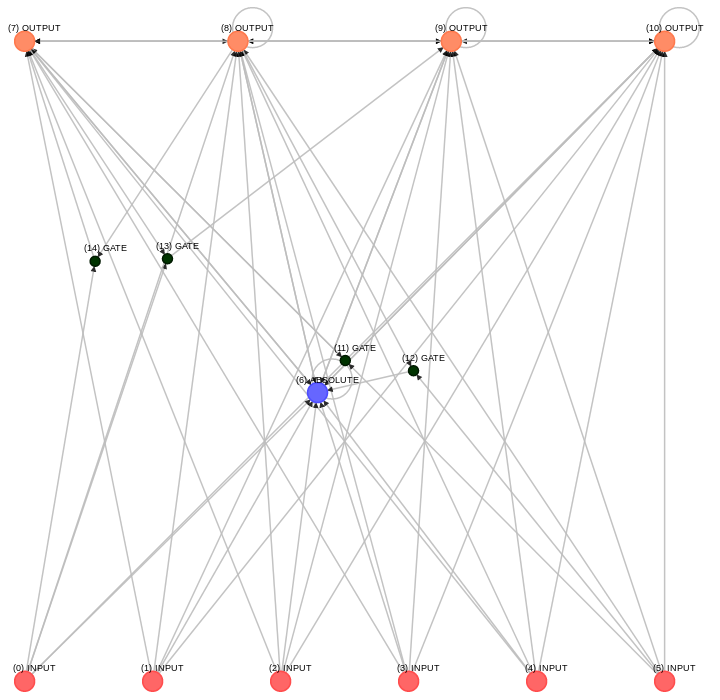
\includegraphics[width=0.7\linewidth]{solutions/IWithObstructions/basic}
	\caption{Neuronová síť - silnice ve tvaru I s překážkami bez rozšíření}
	\label{fig:basic}
\end{figure}
\podsekce{Konfigurace s rozšířeními}
Konfigurace s rozšířením byla schopná překonat větší část druhé obrazovky a dosáhnout přibližně dvojnásobku fitness konfigurace bez rozšíření.
\begin{figure}[H]
	\centering
	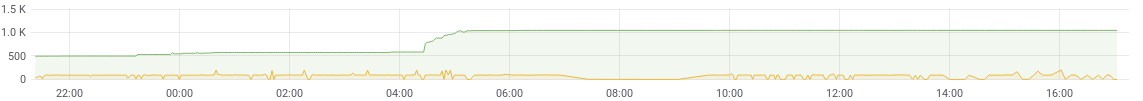
\includegraphics[width=0.7\linewidth]{solutions/IWithObstructions/advancedGraph}
	\caption{Graf průběhu fitness funkce - s překážkami}
	\label{fig:advancedgraph}
\end{figure}
Na výsledné neuronové síti je vidět, že je mnohem komplexnější než kterákoliv předchozí. Je opravdu těžké určit účel jednotlivých neuronů. Zajímavé je, že obsahuje jak neuron s aktivační funkcí absolutní hodnot, jako je tomu v konfiguraci bez rozšíření, tak neuron s aktivační funkcí sigmoid, která může sloužit k dorovnání směru například na základě vstupní rychlosti.

\begin{figure}[H]
	\centering
	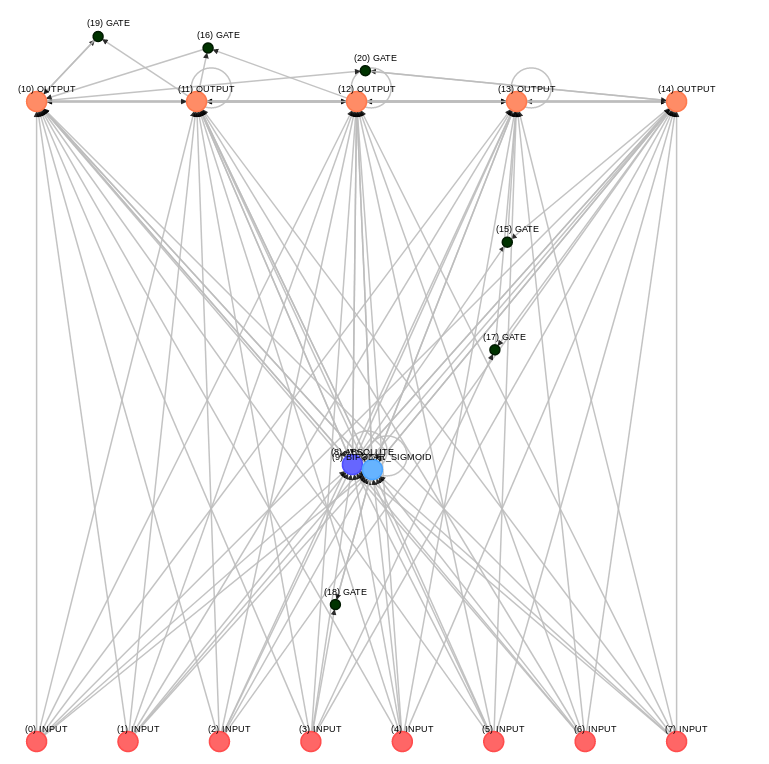
\includegraphics[width=0.7\linewidth]{solutions/IWithObstructions/advanced}
	\caption{Neuronová síť - silnice ve tvaru I s překážkami s rozšířeními}
	\label{fig:advanced}
\end{figure}

\sekce{Třetí stupeň - Okruh}
Stejně jako je tomu u předchozího případu se ani jedné konfiguraci nepovedlo překonat simulační prostředí bez kolize s překážkou.
\podsekce{Konfigurace bez rozšíření}
V základní konfiguraci agent dorazil do vrchní části mapy (dílek ve tvaru obráceného L), kde narazil při pokusu o vytočení překážky.
\begin{figure}[H]
	\centering
	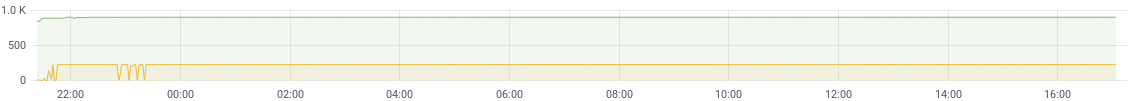
\includegraphics[width=0.5\linewidth]{solutions/Iadvanced/basicGraph}
	\caption{Průběh fitness - Okruh bez rozšíření}
	\label{fig:basicgraph}
\end{figure}
Překvapující je, že toto dokázal bez jakýchkoliv přídavných neuronů.

\begin{figure}
	\centering
	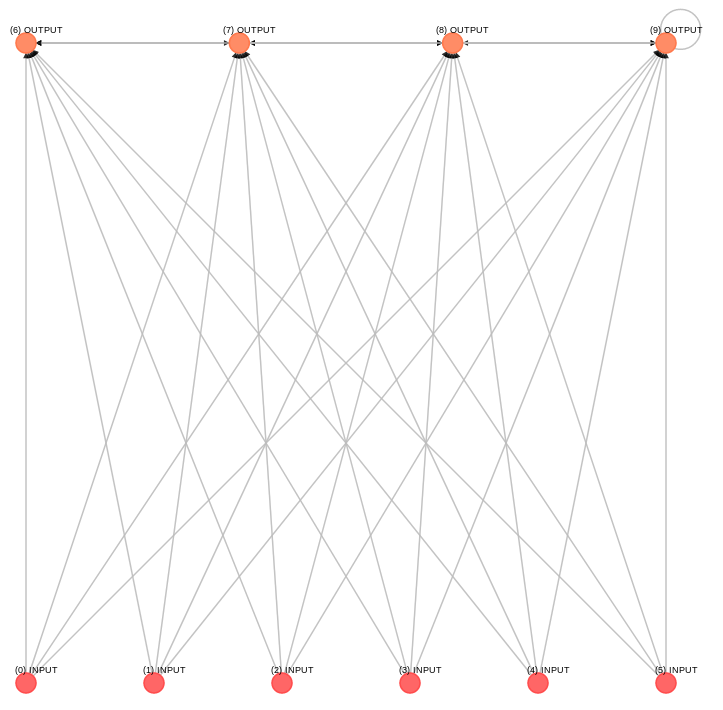
\includegraphics[width=0.5\linewidth]{solutions/Iadvanced/basic}
	\caption{Neuronová síť - Okruh bez rozšíření}
	\label{fig:basic}
\end{figure}

\podsekce{Konfigurace s rozšířením}
Agent si nejprve nacouval do spodní části obrazovky a pak se pokusil pod úhlem překonat vrchní část mapy. Dostal se trochu dál než agent bez rozšíření ale také kolidoval s překážkou.
\begin{figure}[H]
	\centering
	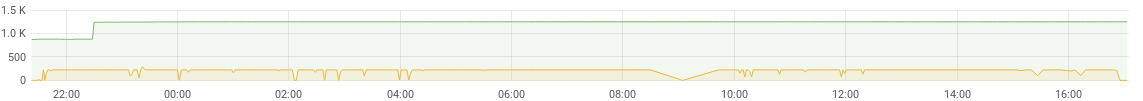
\includegraphics[width=0.5\linewidth]{solutions/Iadvanced/advancedGraph}
	\caption{Průběh fitness funkce - Okruh bez rozšíření}
	\label{fig:advancedgraph}
\end{figure}
Ve výsledné neuronové sítí se nachází neuron s aktivační funkcí SELU. SELU je variace RELU, která by v této konfiguraci mohla sloužit jako implementace výše popsaného manévru.
\begin{figure}[H]
	\centering
	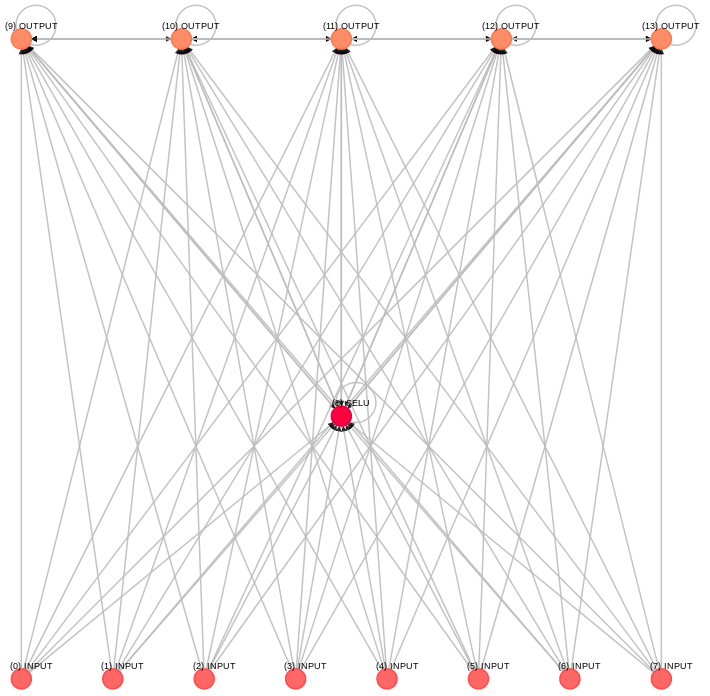
\includegraphics[width=0.5\linewidth]{solutions/Iadvanced/advanced}
	\caption{Neuronová síť - Okruh s rozšířením}
	\label{fig:advanced}
\end{figure}

\sekce{Zhodnocení}
Ačkoliv se výsledným agentům podařilo úspěšně zdolat pouze první překážku, je na provedených experimentech a jejích výsledcích vidět, že lze neuroevoluci použít i pro obtížnější terén. Jediným limitem je časová, případně HW náročnost experimentu.

Experiment odhalil, že algoritmus NEAT ve verzi instinct je schopný produkovat jedince, kteří jsou schopní i komplexních akcí (například manévr popsaný u třetího stupně) a to za použití neuronových sítí, jejíchž architektura je relativně jednoduchá. 

Bylo také zjištěno, že navrhovaná rozšíření značně zlepšují fitness zkoumaného agenta oproti verzi bez rozšíření. Toto lze připsat nejen více dostupným informací ale hlavně větší kontrole nad vozidlem, které neuronové síti nabízí možnost držení volantu ve stejném směru.

Je pravděpodobné, že při dostatečném množství času nebo výpočetního výkonu by bylo možné překonat nejen překážky, které jsou implementovány v této práci ale i překážky, které jsou mnohem složitější. Práce tímto otevírá možností na další, podrobnější testování, které se v ní z časových důvodů nepovedlo.

\kapitola{Možná vylepšení}
Při implementaci aktuálního řešení bylo zjištěno, že řešený problém je mnohem výpočetně náročnější než se při původním návrhu čekalo. Toto vedlo k návrhu distribuovaného řešení, které ovšem sebou nese problémy v rozdílech u výpočtů s desetinou čárkou.

Z tohoto důvodu by experimentu prospělo použití homogenního clusteru. Předešlo by se problémům, které sebou přináší gridový cluster.

Dalším možným rozšířením by bylo spuštění řešení na clusteru s větším výpočetním výkonem. Toto by umožnilo vyzkoušet více experimentů a konfigurací, což by vedlo k lepší představě o  možnostech samotného algoritmu. Navíc by to umožnilo plně využít potenciál, který nabízí oddělený simulační kód (simulace s dynamickými prvky, ...). 

Poslední možností by byla reimplementace existujícího řešení v některém ze systémových jazyků (\textbf{C}, \textbf{C++}, \textbf{Rust}). Došlo by tak k určitému zrychlení výpočtů a bylo by tedy možné vyhodnotit více jedinců na jednom počítači než doposud. 

Grafickou část aplikace by bylo možné rozšířit o různá nastavení, která jsou v tuto chvíli dostupná jen ve zdrojovém kódu aplikace.

\kapitola{Závěr}
Tato práce se zabývala návrhem a  tvorbou prostředí pro simulovaného agenta i jeho řízení pomocí upraveného algoritmu neuroevoluce. Následoval návrh, provedení a zhodnocení experimentů, které byly navrženy tak, aby testovaly možnosti agenta.

Testování agenta proběhlo v různých obtížnostech za různých podmínek. Z provedených testů vyplývá obrovský potenciál metody neuroevoluce, která demonstrovala svojí schopnost řešení komplexních problémů, jako je řízení automobilu a to za použití neuronových sítí. Jejich složitost je oproti konkurenčním řešením, jako je například zpětnovazební učení velmi malá.

Nevýhodou této metody je ovšem její velká časová náročnost, která značně limitovala možnosti této práce a zpomalovala její vývoj.

I přes výše zmíněná omezení se v práci podařilo pomocí výpočetního clusteru vytvořit testovací systém, který je nejen robustní ale i snadno škálovatelný. Použitím většího výpočetního výkonu by tak bylo možné dosáhnout mnohem lepších výsledků a podívat se na limity zkoumané metody do větší hloubky. Bylo například možné plně využít potenciál navrženého řešení pro tvorbu prostředí s dynamickými prvky, jako jsou například další automobily nebo dopravní značení.
